\documentclass[a5paper,11pt]{article}
%Также можно указать системе снизить уровень правил командой \sloppy. В этом случае, все строки будут иметь одинаковую ширину за счет увеличения промежутков между словами и LaTeX выдаст предупреждение о разрежении горизонтального бокса (underfull box). Возвращение к стандартным правилам осуществляется командой \fussy.

% переопределение нумерации

% Этот шаблон документа разработан в 2014 году
% Данилом Фёдоровых (danil@fedorovykh.ru) 
% для использования в курсе 
% <<Документы и презентации в \LaTeX>>, записанном НИУ ВШЭ
% для Coursera.org: http://coursera.org/course/latex .
% Исходная версия шаблона --- 
% https://www.writelatex.com/coursera/latex/5.3

% В этом документе преамбула

% Для корректного использования русских символов в формулах
% пакеты hyperref и настройки, связанные с ним, стоит загуржать
% перед загрузкой пакета mathtext

\usepackage{hyperref}

\hypersetup{				% Гиперссылки
	unicode=true,           % русские буквы в раздела PDF
	pdftitle={Заголовок},   % Заголовок
	pdfauthor={Автор},      % Автор
	pdfsubject={Тема},      % Тема
	pdfcreator={Создатель}, % Создатель
	pdfproducer={Производитель}, % Производитель
	pdfkeywords={keyword1} {key2} {key3}, % Ключевые слова
	colorlinks=true,       	% false: ссылки в рамках; true: цветные ссылки
	linkcolor=red,          % внутренние ссылки
	citecolor=black,        % на библиографию
	filecolor=magenta,      % на файлы
	urlcolor=cyan           % на URL
}

%%% Работа с русским языком
\usepackage{cmap}					% поиск в PDF
\usepackage{mathtext} 				% русские буквы в формулах
\usepackage[T2A]{fontenc}			% кодировка
\usepackage[utf8]{inputenc}			% кодировка исходного текста
\usepackage[english,russian]{babel}	% локализация и переносы
\usepackage{indentfirst}
\frenchspacing

\renewcommand{\epsilon}{\ensuremath{\varepsilon}}
\renewcommand{\phi}{\ensuremath{\varphi}}
\renewcommand{\kappa}{\ensuremath{\varkappa}}
\renewcommand{\le}{\ensuremath{\leqslant}}
\renewcommand{\leq}{\ensuremath{\leqslant}}
\renewcommand{\ge}{\ensuremath{\geqslant}}
\renewcommand{\geq}{\ensuremath{\geqslant}}
\renewcommand{\emptyset}{\varnothing}

%%% Дополнительная работа с математикой
\usepackage{amsmath,amsfonts,amssymb,amsthm,mathtools} % AMS
\usepackage{icomma} % "Умная" запятая: $0,2$ --- число, $0, 2$ --- перечисление

%% Номера формул
%\mathtoolsset{showonlyrefs=true} % Показывать номера только у тех формул, на которые есть \eqref{} в тексте.
%\usepackage{leqno} % Нумереация формул слева

%% Свои команды
\DeclareMathOperator{\sgn}{\mathop{sgn}}

%% Перенос знаков в формулах (по Львовскому)
\newcommand*{\hm}[1]{#1\nobreak\discretionary{}
{\hbox{$\mathsurround=0pt #1$}}{}}

%%% Работа с картинками
\usepackage{graphicx}  % Для вставки рисунков
\graphicspath{{images/}{images2/}}  % папки с картинками
\setlength\fboxsep{3pt} % Отступ рамки \fbox{} от рисунка
\setlength\fboxrule{1pt} % Толщина линий рамки \fbox{}
\usepackage{wrapfig} % Обтекание рисунков текстом

%%% Работа с таблицами
\usepackage{array,tabularx,tabulary,booktabs} % Дополнительная работа с таблицами
\usepackage{longtable}  % Длинные таблицы
\usepackage{multirow} % Слияние строк в таблице

%%% Теоремы
\theoremstyle{plain} % Это стиль по умолчанию, его можно не переопределять.
\newtheorem{theorem}{Теорема}[section]
\newtheorem{proposition}[theorem]{Утверждение}
 
\theoremstyle{definition} % "Определение"
\newtheorem{corollary}{Следствие}[theorem]
\newtheorem{problem}{Задача}[section]
 
\theoremstyle{remark} % "Примечание"
\newtheorem*{nonum}{Решение}

%%% Программирование
\usepackage{etoolbox} % логические операторы

%%% Страница
\usepackage{extsizes} % Возможность сделать 14-й шрифт
\usepackage{geometry} % Простой способ задавать поля
	\geometry{top=25mm}
	\geometry{bottom=35mm}
	\geometry{left=35mm}
	\geometry{right=20mm}
 %
%\usepackage{fancyhdr} % Колонтитулы
% 	\pagestyle{fancy}
 	%\renewcommand{\headrulewidth}{0pt}  % Толщина линейки, отчеркивающей верхний колонтитул
% 	\lfoot{Нижний левый}
% 	\rfoot{Нижний правый}
% 	\rhead{Верхний правый}
% 	\chead{Верхний в центре}
% 	\lhead{Верхний левый}
%	\cfoot{Нижний в центре} % По умолчанию здесь номер страницы

\usepackage{setspace} % Интерлиньяж
%\onehalfspacing % Интерлиньяж 1.5
%\doublespacing % Интерлиньяж 2
%\singlespacing % Интерлиньяж 1

\usepackage{lastpage} % Узнать, сколько всего страниц в документе.

\usepackage{soul} % Модификаторы начертания


\usepackage[usenames,dvipsnames,svgnames,table,rgb]{xcolor}


\usepackage{csquotes} % Еще инструменты для ссылок

%\usepackage[style=authoryear,maxcitenames=2,backend=biber,sorting=nty]{biblatex}

\usepackage{multicol} % Несколько колонок

\usepackage{tikz} % Работа с графикой
\usepackage{pgfplots}
\usepackage{pgfplotstable}




\usepackage{lipsum}
\newcommand{\nn}{0.5pt}

\begin{document}
	\begin{flushright}
		Денисов Егор 8<<М>> класс
		\noindent\rule{0.8\textwidth}{1pt}\\
		\textbf{Вариант II} \\
	\end{flushright}
\sloppy
% так называемая "рыба" образец текста, для получения представления о том, как будет выглядеть текст
%\lipsum[3-35]
\fussy
	\problem Какое из чисел $-5,08; 2\frac56; 0; 1,413$ \textbf{не является} решением неравенства $3x - 4,26 < 0$? Нужное подчеркните.
	\problem Соедините стрелкой неравенство и рисунок, на котором изображено его решение.
	\begin{enumerate}[label = \Roman*:]
			\begin{multicols}{3}
				\item $3x-2\geqslant 10$
				\item $2-3x \geqslant 10$
				\item $10-3x\leqslant2$
		\end{multicols}
	\end{enumerate}
	\begin{figure}[h]
		\begin{center}
			\begin{minipage}[h]{0.45\linewidth}
				1)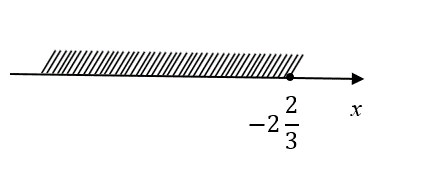
\includegraphics[width=1\linewidth]{1}
				\label{ris:experimoriginal} %% метка рисунка для ссылки на него
			\end{minipage}
			%\hfill
			\begin{minipage}[h]{0.45\linewidth}
				2)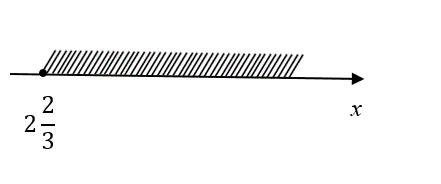
\includegraphics[width=1\linewidth]{2}
				\label{ris:experimcoded}
			\end{minipage}
			\begin{minipage}[h]{0.4\linewidth}
				3)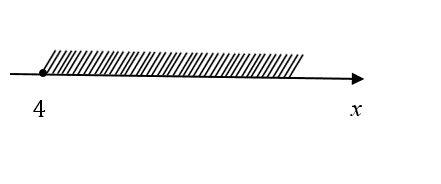
\includegraphics[width=1\linewidth]{3}
				\label{ris:experimcdfoded}
			\end{minipage}
		\end{center}
	\end{figure}
	\setlength{\columnsep}{10ex}
	\problem Изобразите на координатной прямой множество решений данного неравенства и запишите ответ в виде условного обозначения этого множества:
	\begin{enumerate}[label={\realasbuk*)}, ref=\realasbuk*]
		\begin{multicols}{2}
			\item 	$2(4x-5) > 5(x+4)$
			\begin{minipage}[h]{\linewidth}
				\vspace{2ex}
				%\noindent\rule{1\linewidth}{\nn}
				\noindent\rule{1\linewidth}{\nn}
				\noindent\rule{1\linewidth}{\nn}
				\noindent\rule{1\linewidth}{\nn}
				\noindent\rule{1\linewidth}{\nn}
				\textit{Ответ:} \hfill \noindent\rule{0.6\linewidth}{\nn}\\
				%\vspace{1ex}
			\end{minipage}
			\item $\displaystyle\frac{x}4-\frac{x-6}6 +2 \leqslant x$
			\begin{minipage}[h]{1\linewidth}
				\vspace{2ex}
				%\noindent\rule{1\linewidth}{\nn}
				\noindent\rule{1\linewidth}{\nn}
				\noindent\rule{1\linewidth}{\nn}
				\noindent\rule{1\linewidth}{\nn}
				\noindent\rule{1\linewidth}{\nn}
				\textit{Ответ:} \hfill \noindent\rule{0.6\linewidth}{\nn}\\
			\end{minipage}
			\item $2x+4(2x-3)\geqslant\ 12x-11$
			\begin{minipage}[h]{1\linewidth}
				\vspace{2ex}
				\noindent\rule{1\linewidth}{\nn}
				\noindent\rule{1\linewidth}{\nn}
				\noindent\rule{1\linewidth}{\nn}
				\noindent\rule{1\linewidth}{\nn}
				\noindent\rule{1\linewidth}{\nn}
				\textit{Ответ:} \hfill \noindent\rule{0.6\linewidth}{\nn}\\
			\end{minipage}
			\item $16x+20x < 10x -3(4-2x)$
			\begin{minipage}[h]{1\linewidth}
				\vspace{2ex}
				\noindent\rule{1\linewidth}{\nn}
				\noindent\rule{1\linewidth}{\nn}
				\noindent\rule{1\linewidth}{\nn}
				\noindent\rule{1\linewidth}{\nn}
				\noindent\rule{1\linewidth}{\nn}
				\textit{Ответ:} \hfill \noindent\rule{0.6\linewidth}{\nn}
			\end{minipage}
		\end{multicols}
	\end{enumerate}
	\problem
	\begin{enumerate}[label={\realasbuk*)}, ref=\realasbuk*]
		\item При каких значениях $a$ значение выражения $12-7a$ неотрицательно?\\
		\noindent\rule{1\linewidth}{\nn} \\
		\noindent\rule{1\linewidth}{\nn} \\
		\textit{Ответ:} \hfill при $a \in \noindent\rule{0.7\linewidth}{\nn}$
		\item При каких значениях $x$ значение выражения $2-\frac{x}3$
		меньше $-4$?\\
		\noindent\rule{1\linewidth}{\nn} \\
		\noindent\rule{1\linewidth}{\nn} \\
		\textit{Ответ:} \hfill при $a \in \noindent\rule{0.7\linewidth}{\nn}$
		\nopagebreak[4]
		%\newpage
		\item При каких значениях $y$ значение выражения $3-5y$ не больше значения выражения $2(7-y)$?\\ \nopagebreak[4]
		\noindent\rule{\linewidth}{\nn} \\ \nopagebreak[4]
		\noindent\rule{1\linewidth}{\nn} \\ \nopagebreak[4]
		\textit{Ответ:} \hfill при $a \in \noindent\rule{0.65\linewidth}{\nn}$
	\end{enumerate}
	\problem Сколько натуральных решений имеет неравенство:
		\begin{align*}			
			3(x+2)\hm{-}2(x\hm{-}1)\geqslant3x-4?\\
		%\begin{minipage}[h]{\linewidth}
			\vspace{1.8ex}
			\noindent\rule{0.5\linewidth}{\nn}\\
			\noindent\rule{0.5\linewidth}{\nn}\\
			\noindent\rule{0.5\linewidth}{\nn}\\
			\noindent\rule{0.5\linewidth}{\nn}\\
			\noindent\rule{0.5\linewidth}{\nn}\\
			\textit{Ответ:}\hfill \noindent\rule{0.37\linewidth}{\nn}
		%\end{minipage}
	\end{align*}
\end{document}

